\documentclass{article}  % Options: 10pt, 11pt, 12pt


\usepackage{amsmath} 
\usepackage{hyperref}
\usepackage[utf8]{inputenc}
\usepackage{graphicx}
\usepackage{array}
\usepackage{indentfirst}
\DeclareMathAlphabet{\mathcal}{OMS}{cmsy}{m}{n}
\SetMathAlphabet{\mathcal}{bold}{OMS}{cmsy}{b}{n}
\title{Árvore Rubro-Negra}
\author{SERGIO SIVONEI DE SANT'ANA FILHO GRR20242337\\EDUARDO KALUF GRR20241770}
\date{\today} 
\begin{document}
    \maketitle
    
    \section{Apresentação}
    
    \setlength{\parindent}{15pt}

    O objetivo deste trablho é a implementação da árvore Red-Black, também conhecida como Rubro-Negra, utilizando a linguagem C, com base no livro \href{https://computerscience360.wordpress.com/wp-content/uploads/2018/02/algoritmos-teoria-e-prc3a1tica-3ed-thomas-cormen.pdf}{"Algoritmos: Teoria e Prática"} do H. Cormen.
    Esta é uma árvore binária que utiliza um campo de cor a fim de manter a árvore o mais balanceada possível, fazendo com que as operações feitas nela sejam executadas com tempo $\mathcal{O}(\log n)$

    \section{Implementação}

    A implementação foi feita com base nas notas de aula e no próprio livro do Cormen, com modificações a fim de cumprir as especificações do trabalho. A sua construção foi feita do zero, sem utilizar funções de uma BST já implementada, focando em deixar o trabalho mais sucinto e didático.

    Optamos por usar um sentinela que guarda um ponteiro para o nodo raiz e para o nodo \textbf{NIL}. O nodo especial \textbf{NIL} é utilizado para se referir a \textbf{NULL}, sendo então, um nó preto (na Red-Black, ponteiros para \textbf{NULL} são tratados como nós pretos), o qual todos os nodos folhas da árvore apontam.

    Como dito anteriormente, modificações foram feitas para atender aos critérios do trabalho, a função "rb delete", por exemplo, quando deleta a raiz, busca o antecessor (nodo com a chave imediatamente menor que a chave da raiz) para se tornar nova raiz da árvore. No header "rb.h" constam informações mais particulares sobre cada função implementada.

    O algoritmo de busca utilizado no código é a busca binária recursiva, pois a Rubro-Negra se trata de uma árvore binária específica.

    Os comandos aceitos são de inserção e de remoção, representados pelos caracteres "i" e "r" respectivamente, seguindo o formato "instrução valor". 
    \enlargethispage{2\baselineskip}

    Como dito nas espeficicações, a saída é espressada em \textit{ordem} na \textit{stdout}, ordenando por valor, nível e cor, respectivamente. Em caso de valores repetidos, segue ordem crescente de nível, pois chaves idênticas são inseridas à direita, portanto impressas depois, seguindo sempre \textbf{Esquerda \( \rightarrow \) Raiz \( \rightarrow \) Direita}.

    \begin{center}
        \begin{tabular}{>{\raggedleft}p{3cm} c >{\raggedright}p{3cm}}
        \begin{tabular}[t]{@{}l@{}}
        i 10 \\
        i 20 \\
        i 30 \\
        i 20 \\
        i 30 \\
        \end{tabular}
        &
        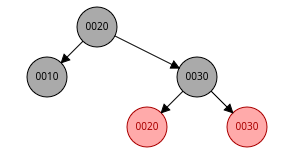
\includegraphics[width=4cm]{redblack.png}
        &
        \begin{tabular}[t]{@{}l@{}}
        10,1,0 \\
        20,0,0 \\
        20,2,1 \\
        30,1,0 \\
        30,2,1 \\
        \end{tabular}
        \end{tabular}
        \end{center}

    \section{Diretórios e Arquivos}

    \begin{itemize}
        \item \texttt{rb.h} \\
        Arquivo header que contém a documentação de cada função utilizada.
        
        \item \texttt{rb.c} \\
        Arquivo de implementação das funções da árvore Red-Black.
        
        \item \texttt{main.c} \\
        Arquivo responsável por receber os comandos passados pelo terminal e chamar as funções correspondentes, gerenciando o fluxo de dados do trabalho.
        
        \item \texttt{Makefile} \\
        Arquivo simples utilizado para compilar e fazer a linkagem do trabalho.
        \begin{itemize}
            \item \texttt{make} \( \rightarrow \) gera o executável \texttt{myrb}
            \item \texttt{make clean} \( \rightarrow \) remove os arquivos gerados pela compilação
        \end{itemize}
        
        \item \texttt{testes} e \texttt{testes.sh} \\
        \texttt{testes.sh} é um script simples que verifica, através dos testes e soluções armazenados no diretório \texttt{testes}, se a árvore implementada está apresentando o comportamento esperado.\\
        O script compila automaticamente o projeto e o executa utilizando o comando \texttt{diff}. Sendo assim, caso nada seja impresso no terminal, todos os testes foram bem-sucedidos.
    \end{itemize}

        
    \section{Conclusão}

    Ao longo deste trabalho, foi possível compreender de forma mais aprofundada como uma árvore Red-Black pode ser implementada, analisando sua estrutura, funcionamento e as vantagens que oferece. Foi possível ver que esse tipo de árvore proporciona uma eficiência ótima nas operações de inserção, remoção e busca. Além disso, sua praticidade de uso em diversas aplicações, como no própio sistema de gerenciamento de arquivos do linux, reforça sua importância como estrutura de dados.

\end{document} 
